To create a TikZ LaTeX diagram that represents the vertex state and the corresponding tetrahedron in the dual simplicial complex, we can use the following code:
```
\documentclass{standalone}
\usepackage{tikz}
\begin{document}
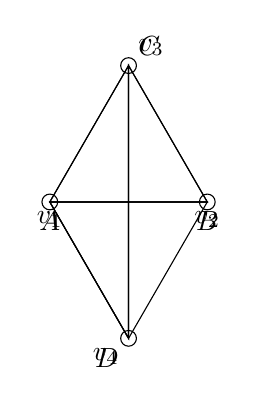
\begin{tikzpicture}
  % Define the vertices of the tetrahedron
  \coordinate (A) at (0,0);
  \coordinate (B) at (2,0);
  \coordinate (C) at (1,1.732);
  \coordinate (D) at (1,-1.732);
  
  % Draw the edges of the tetrahedron
  \draw (A) -- (B) -- (C) -- cycle;
  \draw (A) -- (D) -- (B) -- cycle;
  \draw (C) -- (D) -- (A) -- cycle;
  
  % Label the vertices of the tetrahedron
  \node at (A) [below] {$A$};
  \node at (B) [below] {$B$};
  \node at (C) [above right] {$C$};
  \node at (D) [below left] {$D$};
  
  % Draw the dual simplicial complex
  \draw (A) circle (0.1);
  \draw (B) circle (0.1);
  \draw (C) circle (0.1);
  \draw (D) circle (0.1);
  
  % Label the vertices of the dual simplicial complex
  \node at (A) [below] {$v_1$};
  \node at (B) [below] {$v_2$};
  \node at (C) [above right] {$v_3$};
  \node at (D) [below left] {$v_4$};
  
  % Connect the vertices of the dual simplicial complex
  \draw (A) -- (B) -- (C) -- (D) -- cycle;
\end{tikzpicture}
\end{document}
```
This code will produce a TikZ diagram that shows a tetrahedron with labeled vertices, and its dual simplicial complex with labeled vertices connected by edges. You can adjust the coordinates and labels as needed for your specific problem.